\documentclass{beamer}
\usetheme{Berlin}
\usecolortheme{beaver}
\usepackage{graphicx}
\usepackage[export]{adjustbox}
\usepackage{tikz}
\usetikzlibrary{arrows}
\usepackage{amsmath}
\usepackage{lmodern}% http://ctan.org/pkg/lm

\title{Principles of Digital Data Transmission in Noise}
\subtitle{}
\author[Riccardo \and Eren]{Riccardo~Miccini\inst{1} \and Eren~Can~\inst{1}}
\institute[DTU]
{
	\inst{1}
	Technical University of Denmark\\
	Digital Communication
}
\date{\today}
\subject{Digital Communication}

\tikzstyle{int}=[draw, fill=blue!20]
\tikzstyle{every node}=[font=\tiny]

\begin{document}


	\frame{\titlepage}
	\begin{frame}
		\frametitle{Principles of Digital Data Transmission in Noise}
%		\begin{tikzpicture}[auto,>=latex']
%			\node [int] (a) {ADC};
%			\node (begin) [left of=a,node distance=1cm, coordinate] {a};
%			\node [int] (b) [right of=a] {Line coding};
%			\node [int] (c) [right of=b] {Pulse shaping};
%			\node [int] (d) [right of=c] {Channel};
%			\node [int] (e) [right of=d] {Receiver filter};
%			\node [int] (f) [right of=e] {Thresholder};
%			\node [int] (g) [right of=f] {DAC};
%			\node [coordinate] (end) [right of=g, node distance=1cm]{};
%			\path[->] (begin) edge node {Source} (a);
%			\path[->] (a) edge node {} (b);
%			\path[->] (b) edge node {} (c);
%			\draw[->] (c) edge node {} (d);
%			\draw[->] (d) edge node {} (e);
%			\draw[->] (e) edge node {} (f);
%			\draw[->] (f) edge node {} (g);
%			\draw[->] (g) edge node {} (end);
%		\end{tikzpicture}
	\begin{itemize}
	\item In this chapter, we are concerned with the transmission of information from sources that produce discrete-valued symbols.
	\item	 Throughout this chapter, we will make the assumption that source symbols occur with equal probability. Many discrete-time sources naturally produces symbols with equal probability.
	\end{itemize}
	\end{frame}
	\begin{frame}
		\frametitle{Block Diagram of  Digital Data Tranmission System}
		\begin{figure}
		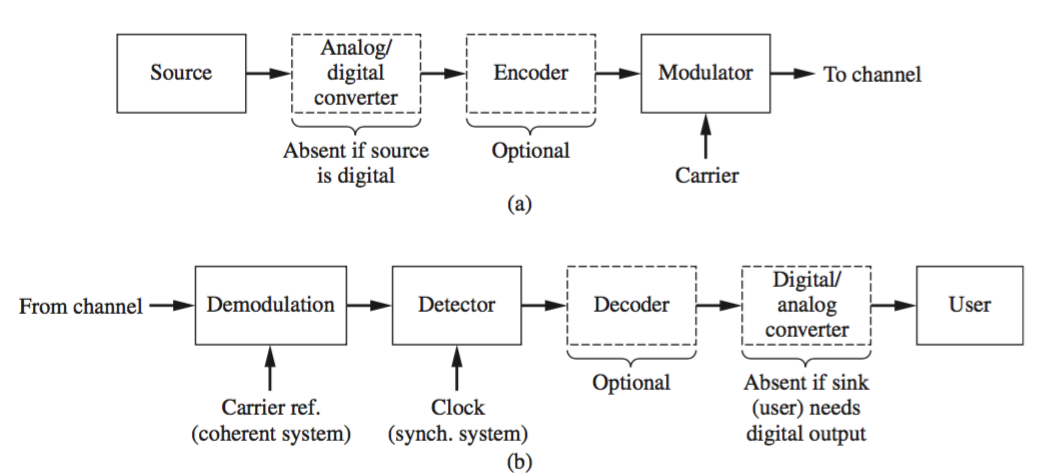
\includegraphics[width=0.8\textwidth]{figure-text7.png}
		\end{figure}
		\end{frame}				
			\begin{frame}
			\begin{itemize}
			\item Whether  a source is purely digital or analog that converted to digital , it may be advantegous to add or remove redundant  digits to the digital signal. This process referred as forward error-correction coding
			\item We can see from the figlure that modulator input take on one of only two possible values. This system will referred as "binary". If it takes M > 2 possible values, system will be referred as M-ary.
			\item Also system will be referred as "coherent" if a local reference is available for demodulation that in phase with the transmitter carrier. Otherwise it will be called "noncoherent".
			\item Also if the system has a periodic signal and synching with transmitted sequence of digital signals than system will be synchronous if not, system will be called asynchronous.
			\end{itemize}
			\end{frame}
			
			\begin{frame}
			\frametitle{Baseband Data Tranmission In White Gaussian Noise}
			\begin{itemize}
			\item  During data transmission, receiver is to decide whether the transmitted signal was A or -A during each bit period.
			\item Practical way of determining this is to pass the signal-pulse noise through a lowpass predectition filter. If the sample greater than zero than A was transmitted if not , -A was transmitted.
			\end{itemize}
			\end{frame}
			
			\begin{frame}
			\begin{figure}
			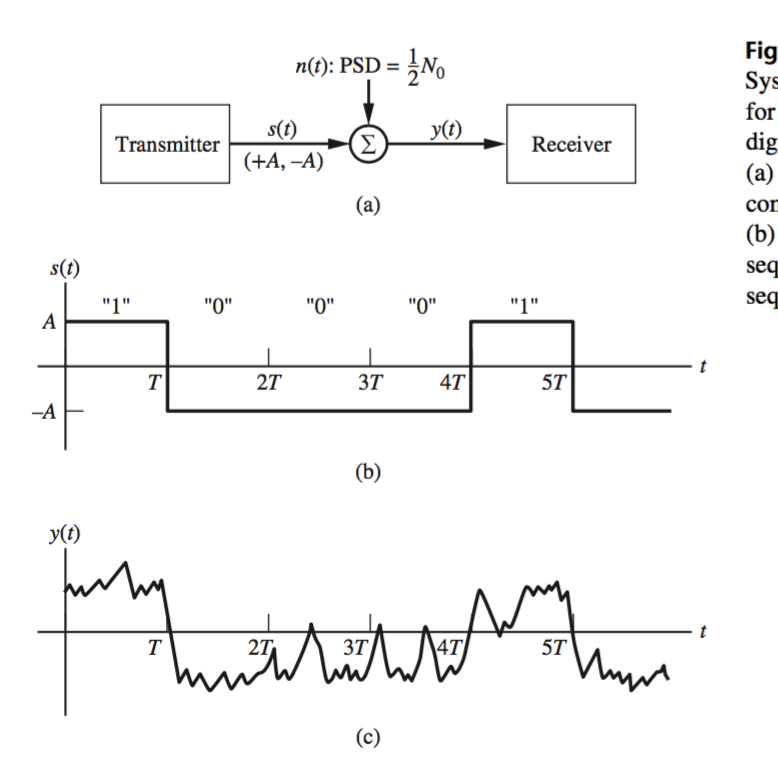
\includegraphics[width=0.5\textwidth]{9.png}
			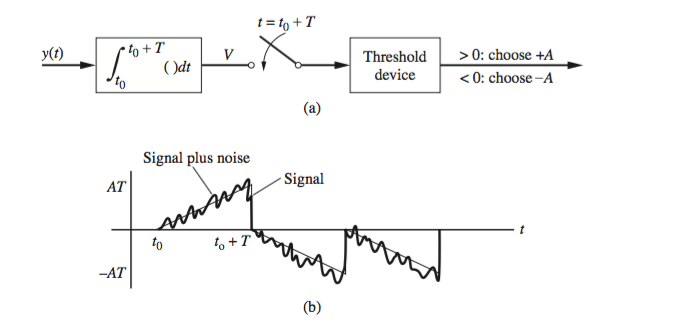
\includegraphics[width=0.5\textwidth]{9-1.png}
			\end{figure}
			\end{frame}
			
			\begin{frame}
			\frametitle{How well does this receiver will perform ?}
			\begin{itemize}
			\item As we discussed before ,useful criterion of performance is probability of error. 
			\item Probability of error through approximation is: $P_E= Q *\sqrt{2*A^2*T/N_o}$
			\item Our important parameters are; $A^2*T/N_0=z$
			\item $E_b$ is called the energy per bit that carries one bit of information.
			\item We also now that rectangular pulse of duration T seconds ahas amplitude spectrum $ATsincTf$ and that $B_p=1/T$ is a rough measure of it's bandwidth. Thus our calculation will become: $E_b/N_o=A^2/N_o*(1/T)=A^2/(N_0*B_p)$. This can be interpreted as the ratio of signal power to noise power in the signal bandwidth.
			\end{itemize}
			\end{frame}
			
			\begin{frame}
			\frametitle{Plot of of $P_E$ versus z}
			\begin{figure}
			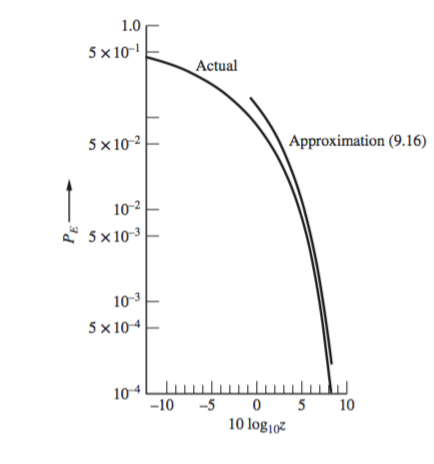
\includegraphics[width=0.5\textwidth]{P_E graph.png}
			\end{figure}
			\end{frame}
			\end{document}
			
